The $256^3$ run has particle mass $4.15\times10^{10}$\,\Msunh{}, $\epsilon_G = 26$\,$h^{-1}$kpc and
$\epsilon_P = 13$\,$h^{-1}$kpc. Both runs and the full halo pipeline completed (Table~\ref{tab:run256}).

\begin{table}[H]
\centering\small
\begin{tabular}{@{}lll@{}}
\toprule
stage & \gad{} & \pkd{} \\
\midrule
simulation & 2.9\,h, 64 MPI ranks, 101 snapshots, 63\,GB & 2.6\,h, 64 threads, 101 outputs, peak memory 14\,GB \\
Rockstar & 29\,min, 40\,658 halos at $z=0$ & 29\,min, 39\,883 halos at $z=0$ \\
consistent-trees & 10\,min, 94 hlists ($z \le 7.8$) & 11\,min, 94 hlists \\
VAHC (grid $512^3$) & 2.3\,h with 8 processes (peak 168\,GB) & 3.5\,h with 8 processes \\
comparison & \multicolumn{2}{l}{29\,min (23 outputs, peak 9\,GB); stacks 3--13\,s per code and output} \\
\bottomrule
\end{tabular}
\caption{$256^3$ jobs on pawna. consistent-trees skips the 7 earliest catalogues ($<20000$ bytes, production
threshold), so at $z > 7.8$ the halo comparison uses the Rockstar catalogues.}
\label{tab:run256}
\end{table}

\subsection{Particles: potential, positions, velocities}

\begin{table}[H]
\centering\small
\begin{tabular}{@{}rrcccccccc@{}}
\toprule
out & $z$ & corr$(\phi)$ & $\frac{{\rm rms}\,\Delta\phi}{{\rm rms}\,\phi}$ & FFT$_{x}$ & offset & med $|\Delta x|$ & 90\% $|\Delta x|$ & med $|\Delta v|$ & corr$(v)$ \\
 & & & & & \kms & \Mpch & \Mpch & km\,s$^{-1}$ & \\
\midrule
0 & 11.98 & 0.999994 & 0.006 & 0.001 & $+849$ & 0.0032 & 0.006 & 0.9 & 1.0000 \\
19 & 2.96 & 0.999802 & 0.021 & 0.015 & $-640$ & 0.014 & 0.055 & 2.0 & 0.979 \\
46 & 1.00 & 0.995549 & 0.095 & 0.085 & $-966$ & 0.045 & 0.259 & 11.9 & 0.908 \\
64 & 0.50 & 0.990111 & 0.142 & 0.129 & $-1192$ & 0.074 & 0.367 & 37.5 & 0.867 \\
100 & 0.00 & 0.976212 & 0.220 & 0.199 & $-1093$ & 0.116 & 0.517 & 69.8 & 0.791 \\
\bottomrule
\end{tabular}
\caption{$256^3$, particle by particle (columns as in Table~\ref{tab:p32}). \pkd{}'s removed self-term is
$-2.9\times10^5$\,\kms{} at $z=12$ and $-2.25\times10^4$ at $z=0$.}
\label{tab:p256}
\end{table}

\begin{itemize}
\item \textbf{Before structure forms the two codes agree very closely.} At $z=12$ the potentials correlate to
$1-6\times10^{-6}$ with 0.6\% rms difference. That is better than either code agrees with the FFT
reference ($1-6\times10^{-5}$), so it is limited by the reference, not by the codes. Particles are 3\,$h^{-1}$kpc
apart (0.12\,$\epsilon_G$) and velocities agree to 0.9\,km\,s$^{-1}$.
\item \textbf{The difference then grows with nonlinear structure}, to 2\% rms at $z = 3$, 10\% at $z=1$ and 22\% at
$z=0$ (25\% at $32^3$). From $z\approx3$ on, 75--90\% of it is accounted for by the particles being in different
places: the FFT potentials of the two sets of positions differ by 0.73 (at $z=3$) to 0.90 (at $z=0$) of the rms
$\Delta\phi$ (Fig.~\ref{fig:pvz}). The force solvers themselves agree far better than the rms suggests (see also the matched
halos below).
\item \textbf{The zero points agree} to $\le 1.2\times10^3$\,\kms{} after removing \pkd{}'s self-term, about 0.1\%
of rms $\phi$. The \texttt{.pkc} potential matches \pkd{}'s HDF5 to 0.5\,\kms{} (half the quantisation step) at
every output.
\item \textbf{Positions and velocities.} At $z=0$ the median particle separation is 0.116\,\Mpch{} (4.5
$\epsilon_G$; 15\% of the mean interparticle spacing) and the 90th percentile 0.52\,\Mpch. Velocities split into two
populations (Fig.~\ref{fig:p256}):
  \begin{itemize}
  \item particles outside halos, $|\Delta v| \approx 3$\,km\,s$^{-1}$;
  \item particles inside halos, whose orbits are chaotic, $|\Delta v| \sim 100$--300\,km\,s$^{-1}$.
  \end{itemize}
  The median is 70\,km\,s$^{-1}$ and the rms 380\,km\,s$^{-1}$. The rms velocities of the two runs differ by 0.7\% at
$z=0$.
\end{itemize}

\begin{figure}[H]
\centering
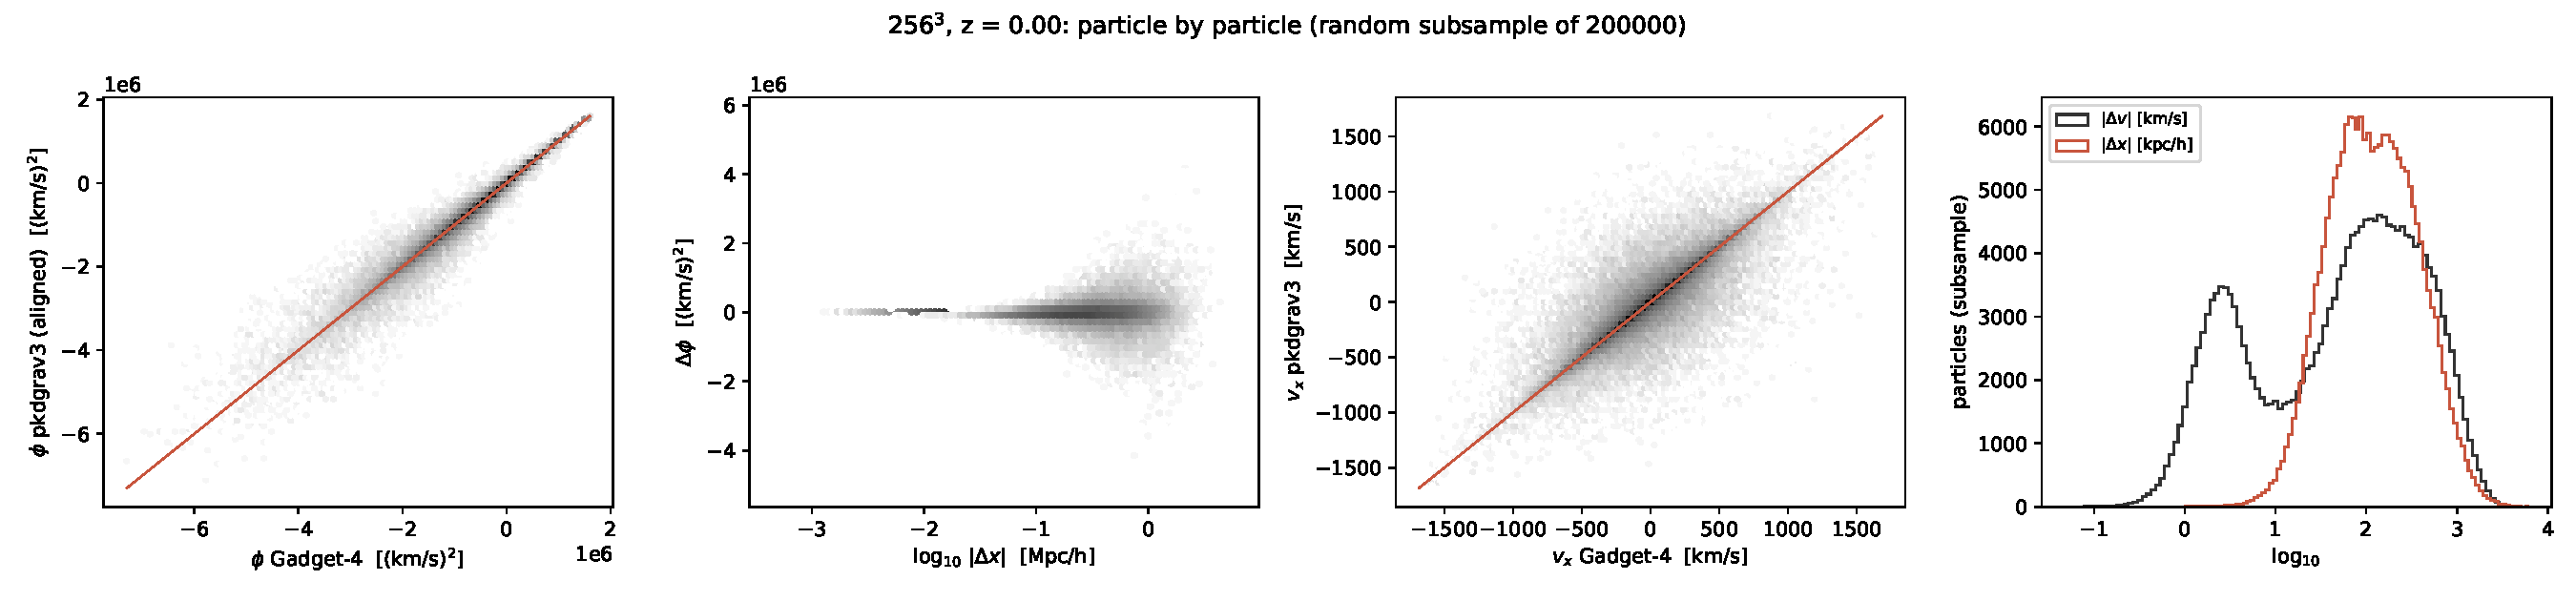
\includegraphics[width=\textwidth]{figs/particles_256_z0.pdf}
\caption{$256^3$, $z=0$, a random 200\,000 particles: potentials, $\Delta\phi$ against separation, $v_x$, and the
distributions of $|\Delta v|$ and $|\Delta x|$. The bimodal $|\Delta v|$ separates field particles from halo
particles.}
\label{fig:p256}
\end{figure}

\subsection{Halo catalogues and VAHC}

At $z=0$ there are 36\,043 (\gad{}) and 35\,404 (\pkd{}) host halos; 28\,484 are matched one to one.
\begin{itemize}
\item \textbf{Mass function} (Fig.~\ref{fig:mf256}). The $M_{\rm vir}$ functions agree within 2--3\% (and within
Poisson errors) from $10^{12}$ to $10^{14.5}$\,\Msunh{} at every redshift. Below $\sim 10^{12}$\,\Msunh{} (30
particles) \pkd{} has 5\% fewer halos at $5\times10^{11}$ and 13\% fewer at $2\times10^{11}$.
\item \textbf{The $V_{\max}$ function differs more.} \pkd{} has 14--17\% fewer halos at 100--160\,km\,s$^{-1}$ and
13--19\% more at 300--600\,km\,s$^{-1}$ ($z=0$; about half as much at $z=1$). This follows from the halo structure
below.
\item \textbf{Matched halos} (Fig.~\ref{fig:match256}). The matched fraction is $\ge 96\%$ above
$3\times10^{12}$\,\Msunh{}, 79\% at $10^{12}$--$3\times10^{12}$ and 45\% at
$3\times10^{11}$--$10^{12}$.
  \begin{itemize}
  \item \emph{Masses} agree: median ratio 1.00 above $10^{12}$\,\Msunh{}, with 16--84\% range $\pm12\%$ at $10^{12}$
  narrowing to $\pm2\%$ at $10^{14}$.
  \item \emph{\pkd{} halos are more concentrated}: $R_{\rm vir}/r_s$ is higher by 21--26\% at
  $10^{12}$--$10^{13}$\,\Msunh{}, 9\% at $3\times10^{13}$ and 3\% above $10^{14}$. Their $V_{\max}$ is 2--5\% higher.
  \item \emph{Shapes}: above $3\times10^{12}$\,\Msunh{} \pkd{} halos are somewhat rounder, with $c/a$ higher by 6--17\%.
  \item \emph{Spin} agrees (median ratio 0.99--1.02).
  \item \emph{Centres and bulk velocities}: the median centre offset is 0.24\,$R_{\rm vir}$ at $10^{12}$, 0.11 at
  $10^{13}$ and 0.03 at $3\times10^{14}$\,\Msunh{}. Bulk velocities differ by 15--80\,km\,s$^{-1}$ (median).
  \end{itemize}
  The higher central density is consistent with \pkd{}'s smaller effective softening ($2\epsilon_P = \epsilon_G$
  against \gad{}'s spline support $2.8\epsilon_G$). It is largest at $10^{12}$--$10^{13}$\,\Msunh{}, where
  $r_s$ is only a few $\epsilon_G$.
\item \textbf{VAHC.} The halo-by-halo bias $b_1$ is measured from the density field at $k<0.1\,h$\,Mpc$^{-1}$, which
the two runs share. It is identical (correlation 1.0000; rms difference 0.010, against a halo-to-halo scatter of 3.4).
The tidal eigenvalue $\lambda_1$ correlates at 0.98 with $R = 4R_{200b}$ smoothing (rms difference 1.0, scatter 5.4)
and at 0.94 with $2R_{200b}$, where the halo's own surroundings, which differ in detail, matter more.
\item \textbf{Potential of matched halos} (Fig.~\ref{fig:hpot256}).
  \begin{itemize}
  \item \pkd{}'s $\phi_{\min}$ is 4--9\% deeper (median per mass decade at $z=0$), the mean potential of the 10\% most
  bound particles 4--6\% deeper, and $\langle\phi\rangle$ within $R_{\rm vir}$ 1--2\% deeper. This is the same
  central-density difference.
  \item For the same particles, \pkd{}'s mean potential of each \gad{} halo's members agrees with \gad{}'s to
  0.1--0.5\%. That is the cleanest test of the two potentials, free of halo-finder and centring differences.
  \end{itemize}
\end{itemize}

\begin{figure}[H]
\centering
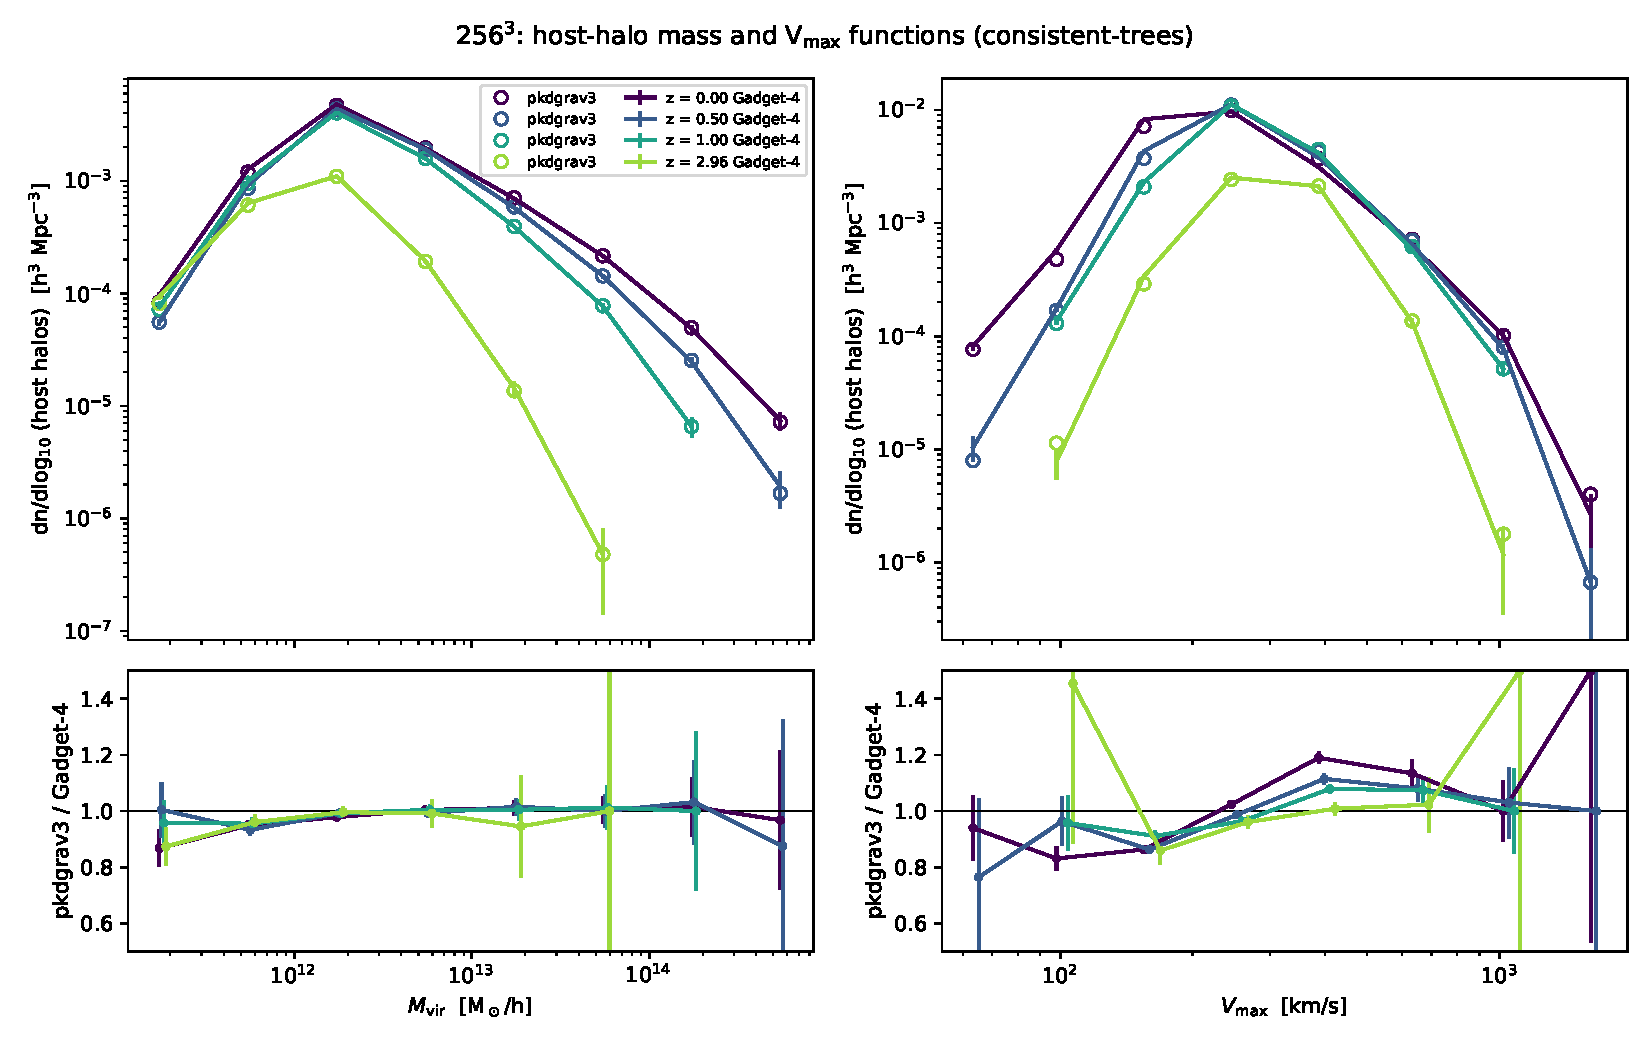
\includegraphics[width=0.85\textwidth]{figs/halo_mf_256.pdf}
\caption{$256^3$: host-halo $M_{\rm vir}$ and $V_{\max}$ functions from the consistent-trees catalogues of the two
codes at $z\approx3$, 1, 0.5 and 0 (lines with errors: \gad{}; circles: \pkd{}). Bottom: ratio with Poisson errors.}
\label{fig:mf256}
\end{figure}

\begin{figure}[H]
\centering
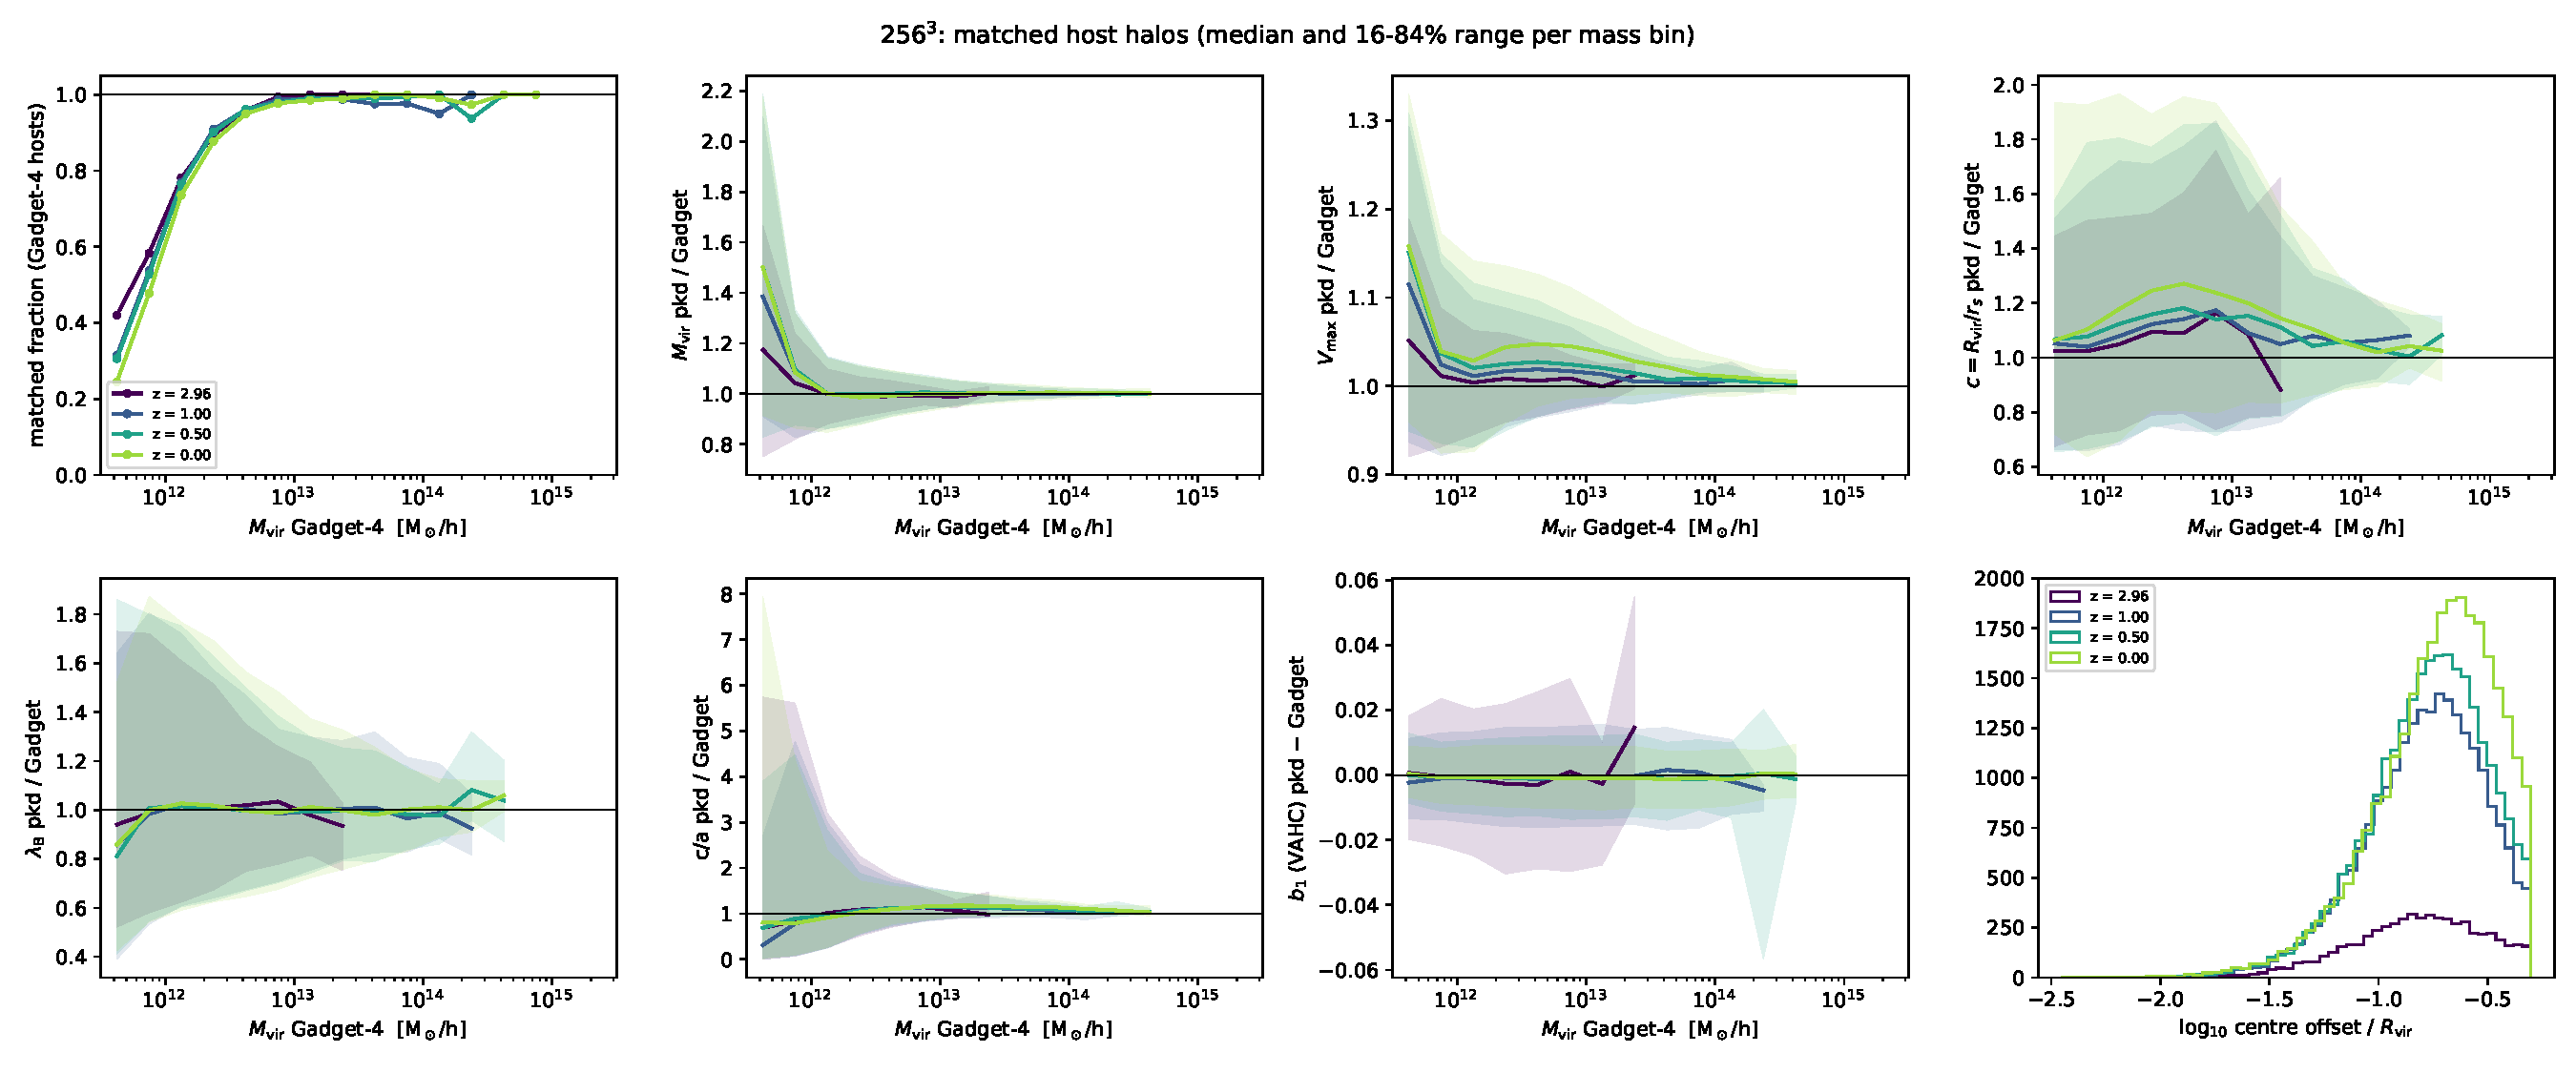
\includegraphics[width=\textwidth]{figs/halo_match_256.pdf}
\caption{$256^3$: matched host halos. Matched fraction, and per \gad{} mass bin the median (line) and 16--84\% range
(band) of \pkd{}/\gad{} for $M_{\rm vir}$, $V_{\max}$, concentration, spin and $c/a$; the difference of the VAHC
bias $b_1$; and the distribution of centre offsets.}
\label{fig:match256}
\end{figure}

\begin{figure}[H]
\centering
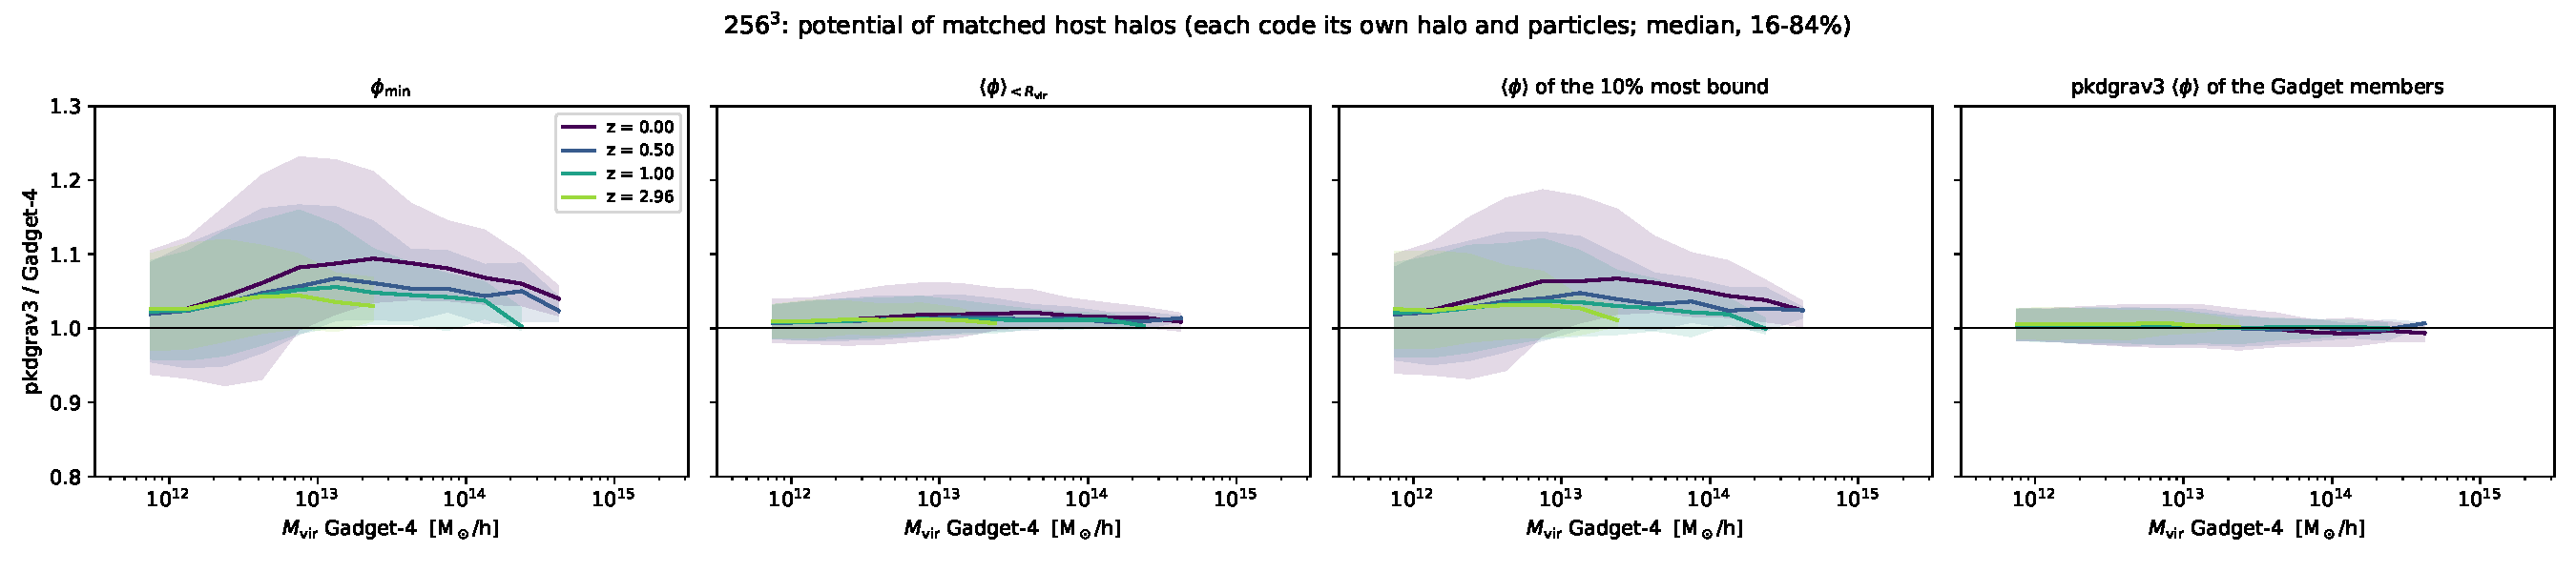
\includegraphics[width=\textwidth]{figs/halo_potential_256.pdf}
\caption{$256^3$: potential of matched host halos, \pkd{}/\gad{}. Each code uses its own halo and its own particles
within $R_{\rm vir}$, except in the last panel, where \pkd{}'s potential is evaluated for the \gad{} halo's member
particles (same IDs).}
\label{fig:hpot256}
\end{figure}

\subsection{Stacked potential around halos}

Figures~\ref{fig:s256}--\ref{fig:xi256} come from the notebook \fp{stack_potential.ipynb}. Each code uses its own
host halos in four $M_{\rm vir}$ bins. At $z=0$ these hold 13\,375 / 3\,181 / 525 / 78 halos in \gad{}
($2\times10^{12}$--$10^{13}$, $10^{13}$--$5\times10^{13}$, $5\times10^{13}$--$2\times10^{14}$, $>2\times10^{14}$\,\Msunh)
and the same within 1\% in \pkd{}. Differences carry the paired jackknife error: the two codes' differences
over the same sub-cubes, which removes the shared large-scale (sample) variance. The dilution uses the same particle
IDs in both codes, so the subsampling noise of the outer shells cancels as well.

\begin{itemize}
\item \textbf{Shape.} $\langle\phi\rangle(r)$ is deepest at the centre, from $-5\times10^{5}$\,\kms{} in the lowest
bin to $-5\times10^6$ in the highest. In the low-mass bins it has a second minimum at 1--3\,\Mpch: small halos
often sit near larger ones. It is still $\approx -6\times10^5$\,\kms{} at 50\,\Mpch, because halos live in
large-scale potential wells. The scatter $\sigma_\phi$ in a shell, $(5$--$10)\times10^5$\,\kms, is set by the
large-scale potential and is much larger than any code difference.
\item \textbf{\pkd{} $-$ \gad{}.}
  \begin{itemize}
  \item Inside $\sim0.1$\,\Mpch{} \pkd{} is deeper: by 3--5\% at 0.05\,\Mpch{} (3--6 paired errors), and by up to
  $3\times10^5$\,\kms{} (6\%) at 0.02\,\Mpch{} in the most massive bin. This is the softening and concentration
  difference.
  \item From 0.2 to 50\,\Mpch{} the mean potentials agree to 1--2\% (mostly within 2 paired errors) at all four
  redshifts. In units of the shell scatter that is $|\Delta\langle\phi\rangle| \le 0.02\,\sigma_\phi$.
  \end{itemize}
\item \textbf{\texttt{.pkc} = HDF5.} \pkd{}'s compressed snapshots give the same stacks as its HDF5 snapshots at all
radii.
\item \textbf{Matter around the halos} (Fig.~\ref{fig:xi256}). $1+\xi_{hm}$ agrees within 2\% beyond 0.1\,\Mpch.
Inside, \pkd{} has more mass: +50\% at 0.02\,\Mpch{} in the lowest bin, falling to $\lesssim 10\%$ in the
highest.
\end{itemize}

\begin{figure}[H]
\centering
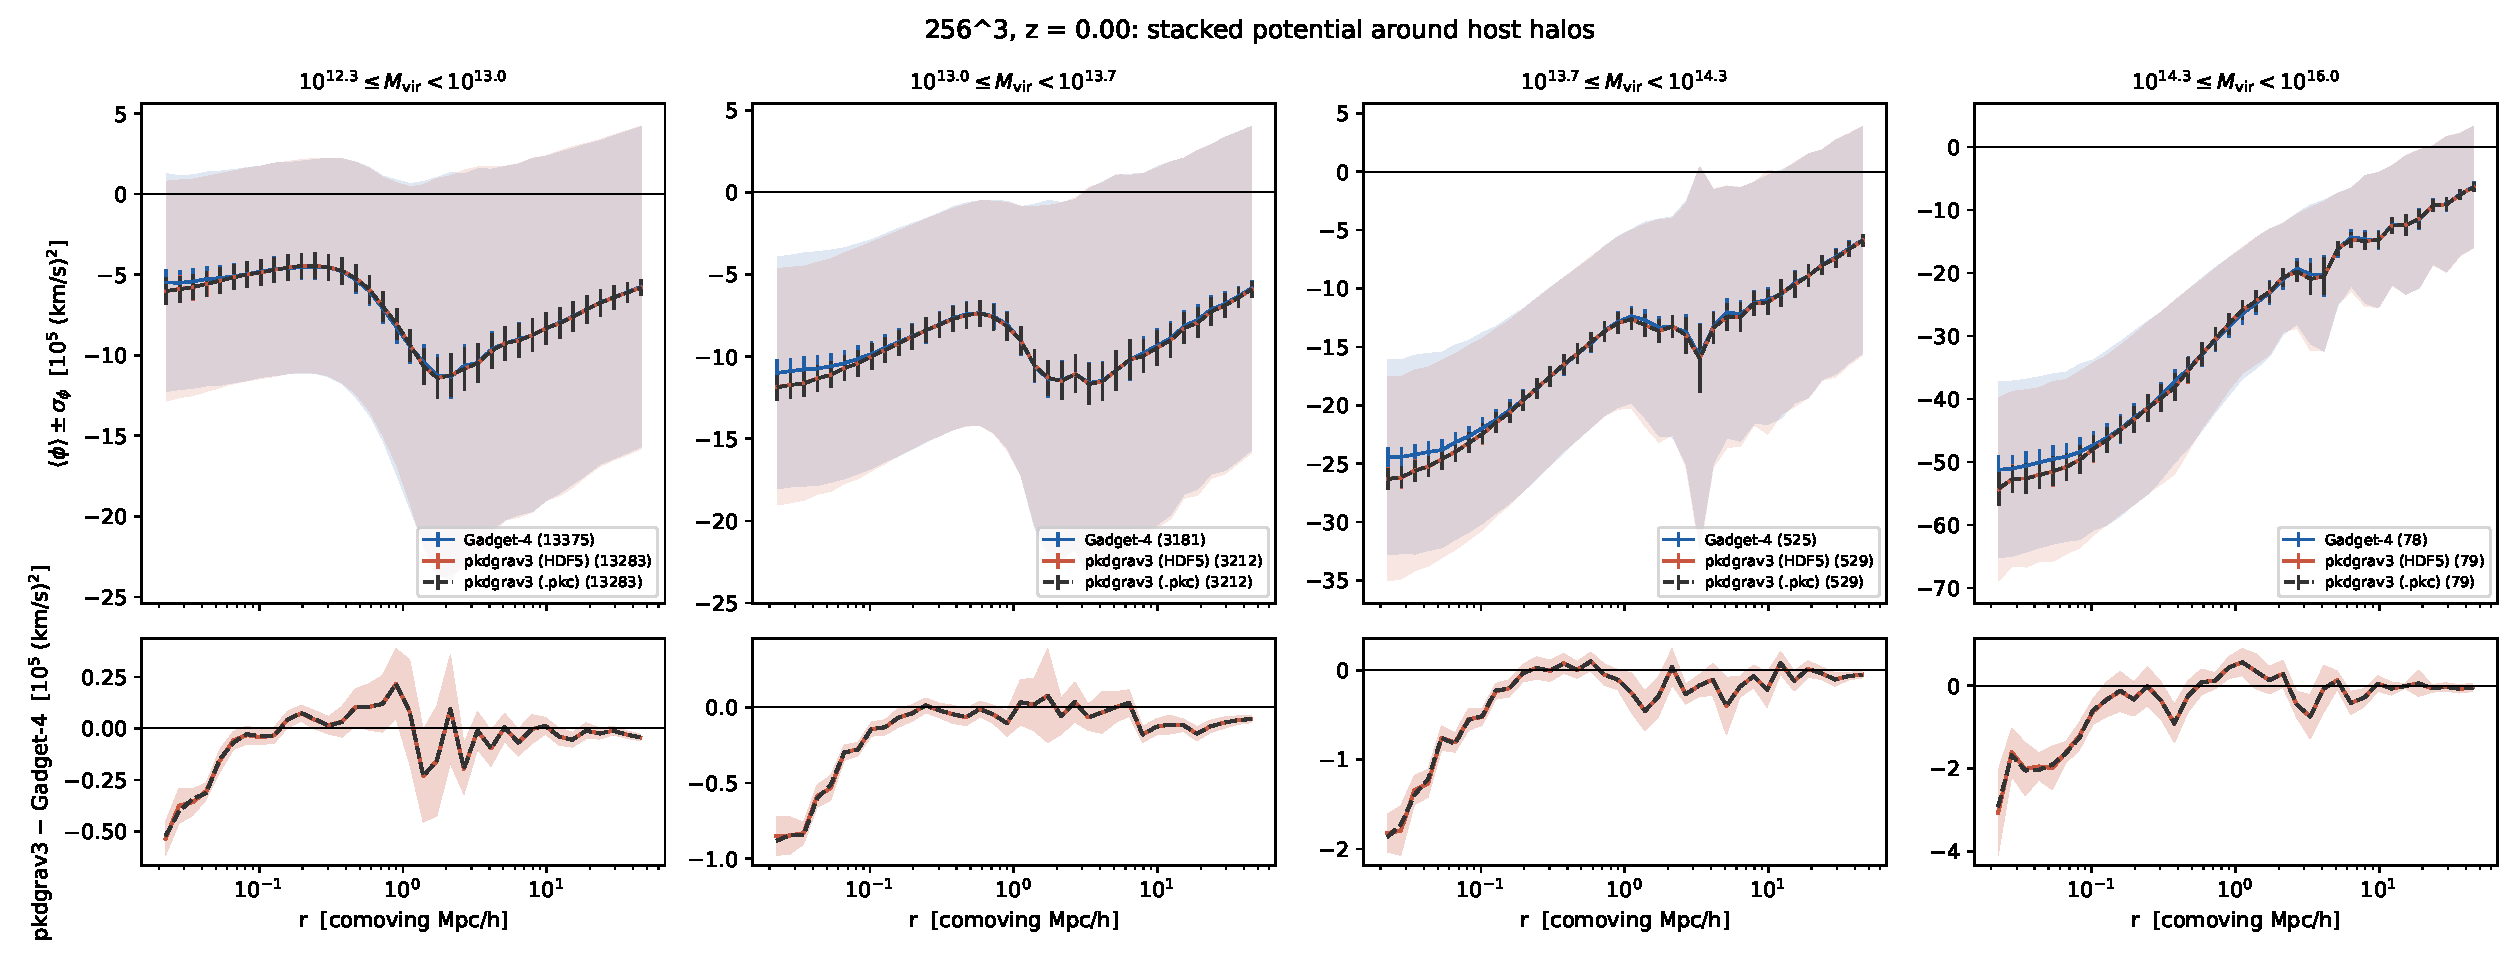
\includegraphics[width=\textwidth]{figs/stack_256_out100.pdf}
\caption{$256^3$, $z=0$: stacked potential around host halos in four $M_{\rm vir}$ bins out to 50\,\Mpch{} (number of
halos in the legend). Lines with error bars: mean and jackknife error; bands: $\pm\sigma_\phi$. Bottom: \pkd{} $-$
\gad{} (solid: HDF5, dashed: \texttt{.pkc}) with the paired jackknife error.}
\label{fig:s256}
\end{figure}

\begin{figure}[H]
\centering
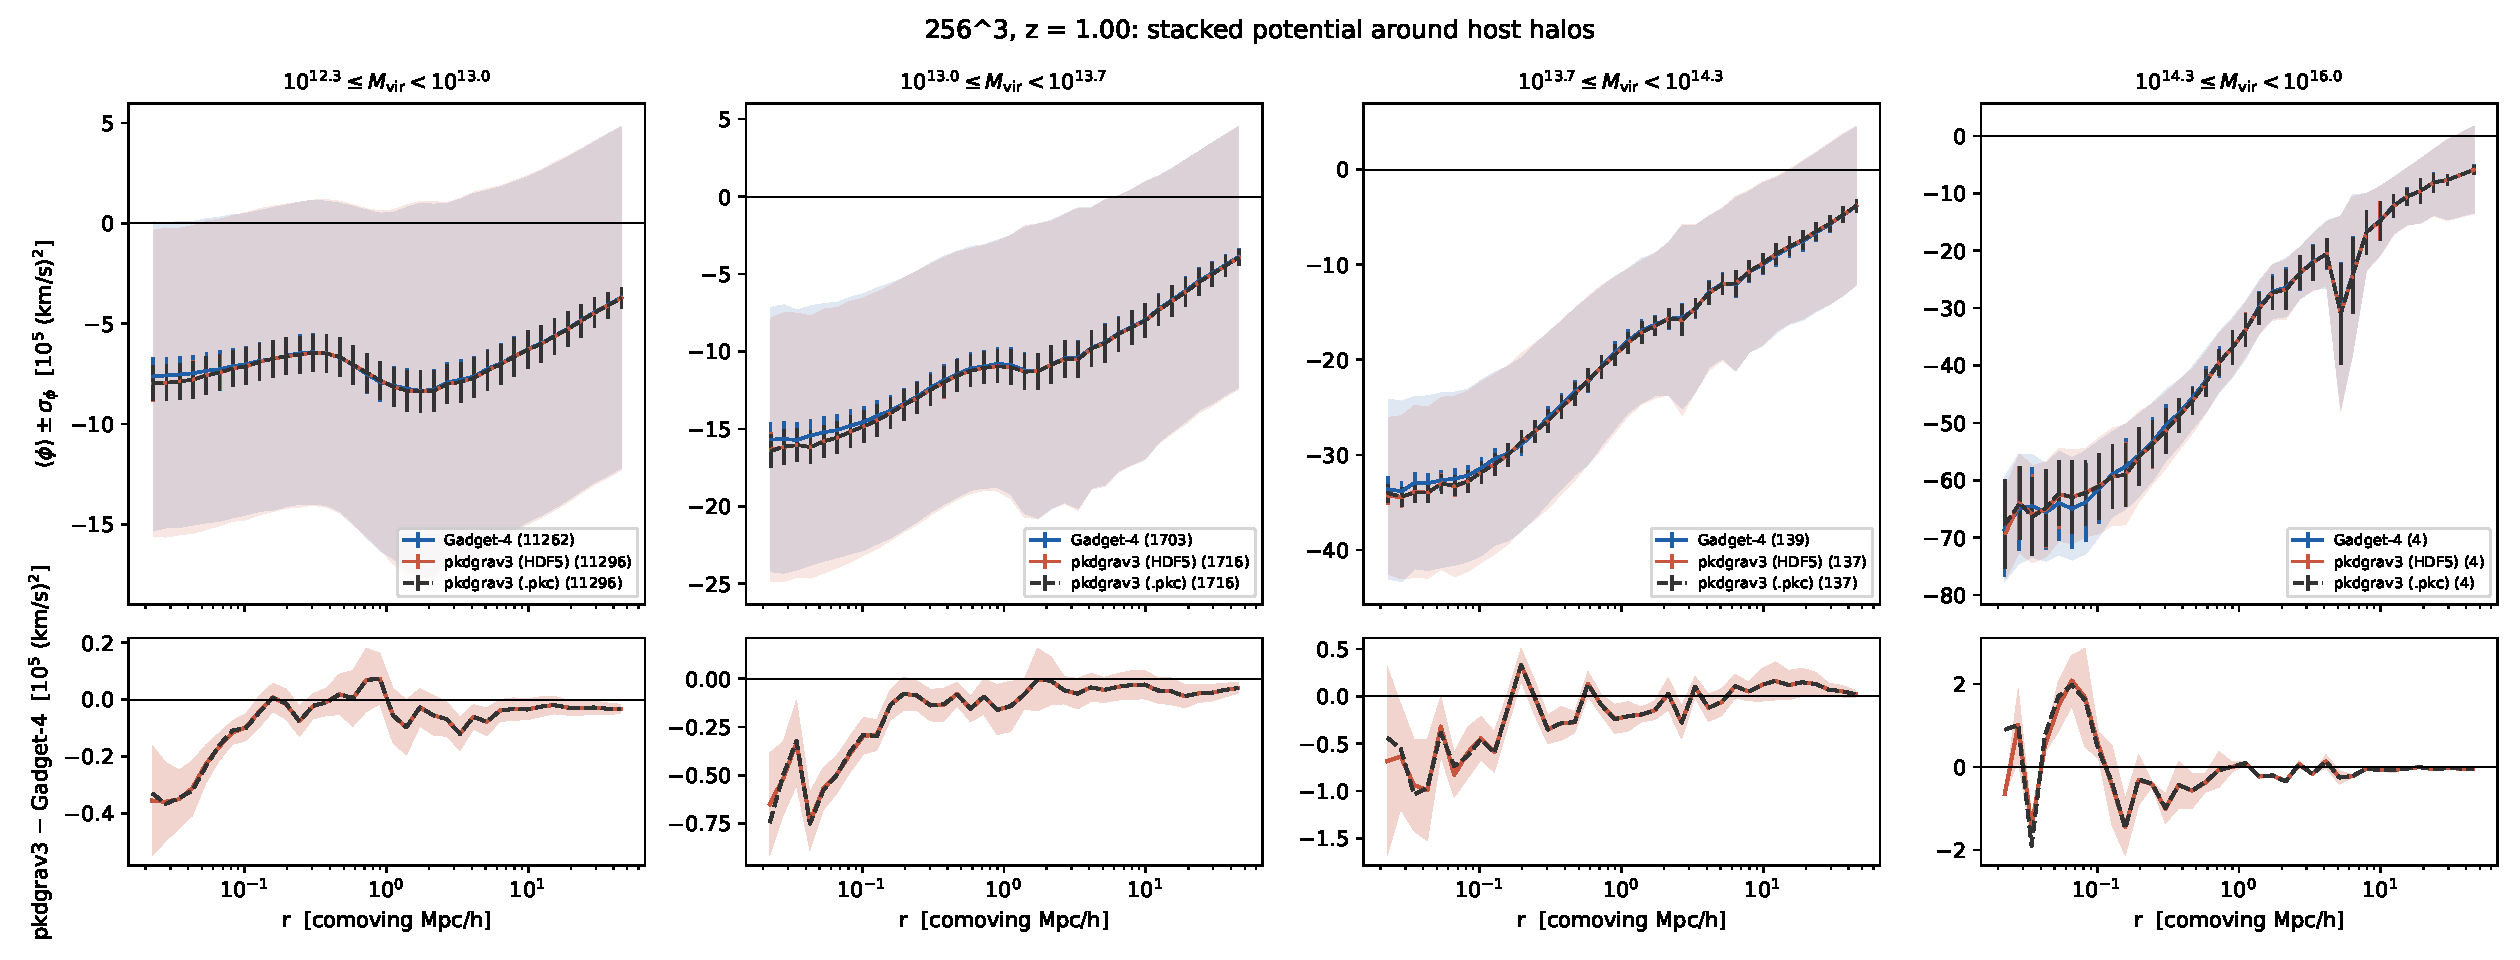
\includegraphics[width=\textwidth]{figs/stack_256_out046.pdf}
\caption{As Fig.~\ref{fig:s256} at $z = 1$.}
\end{figure}

\begin{figure}[H]
\centering
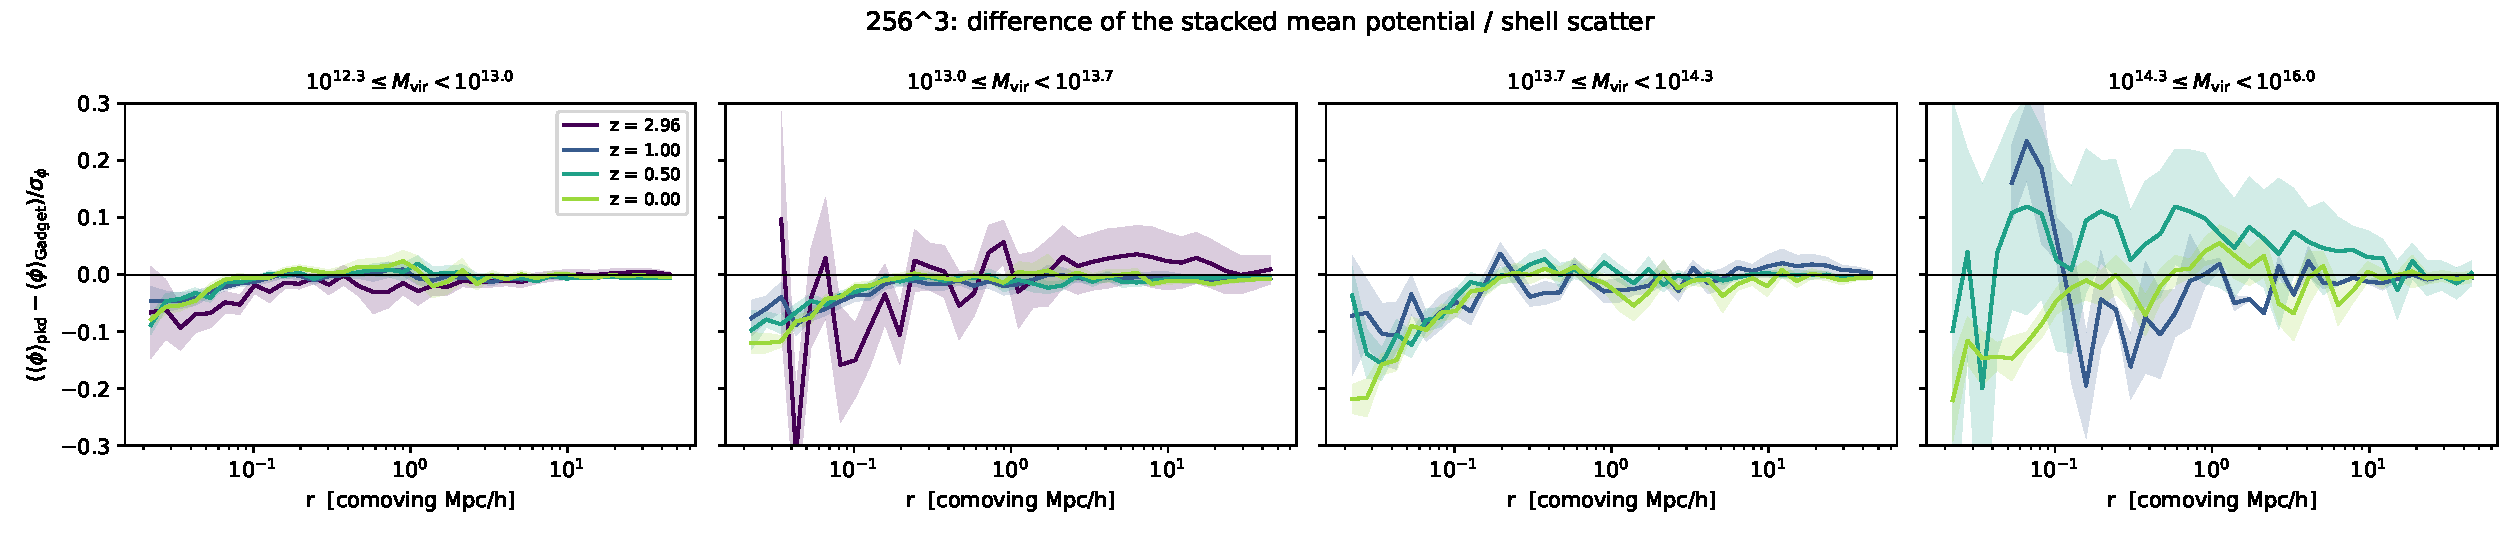
\includegraphics[width=\textwidth]{figs/stack_rel_256.pdf}
\caption{$256^3$: $\Delta\langle\phi\rangle/\sigma_\phi$ at $z \approx 3$, 1, 0.5 and 0, with the paired jackknife
error.}
\label{fig:srel256}
\end{figure}

\begin{figure}[H]
\centering
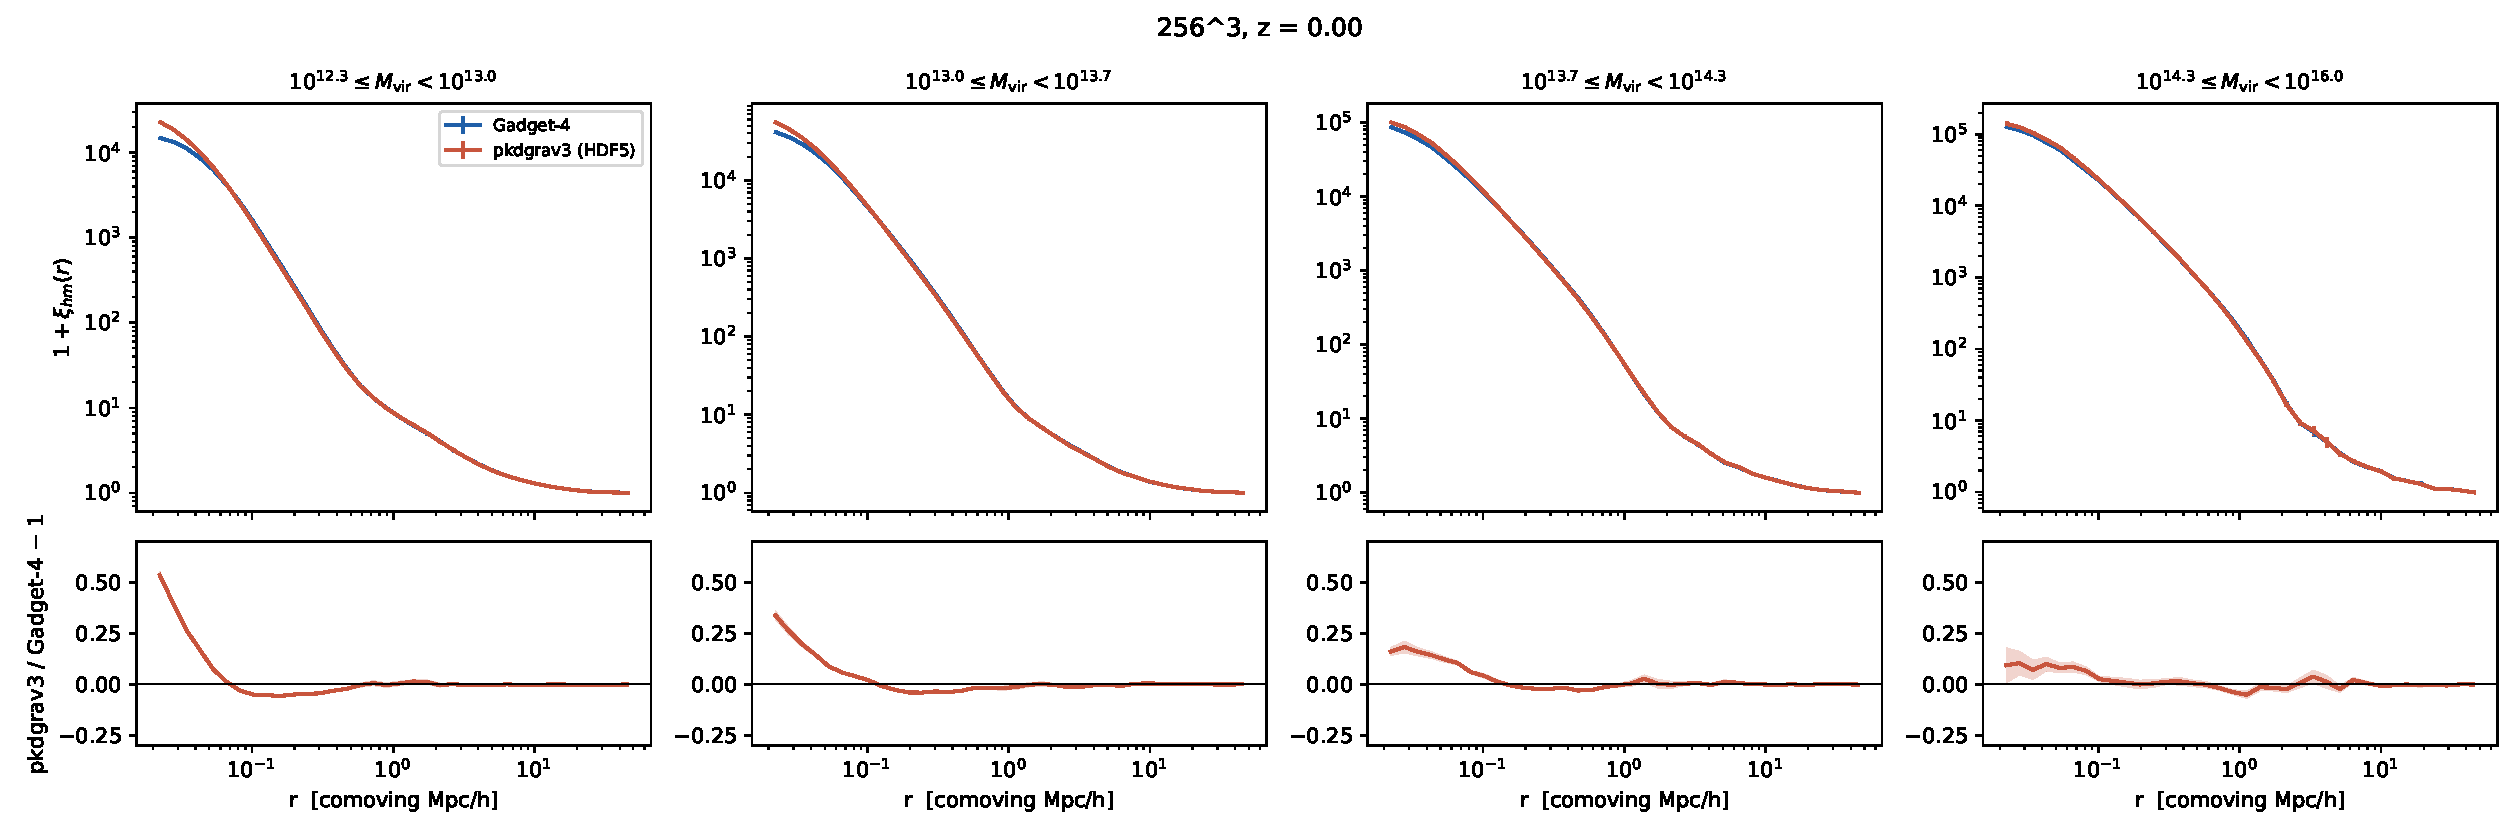
\includegraphics[width=\textwidth]{figs/xihm_256.pdf}
\caption{$256^3$, $z=0$: halo--matter cross-correlation from the same stacks; bottom: \pkd{}/\gad{} $-1$ with the
paired jackknife error.}
\label{fig:xi256}
\end{figure}
